\section{Appendix}\label{appendix}

\begin{figure}[H]
	\centering
	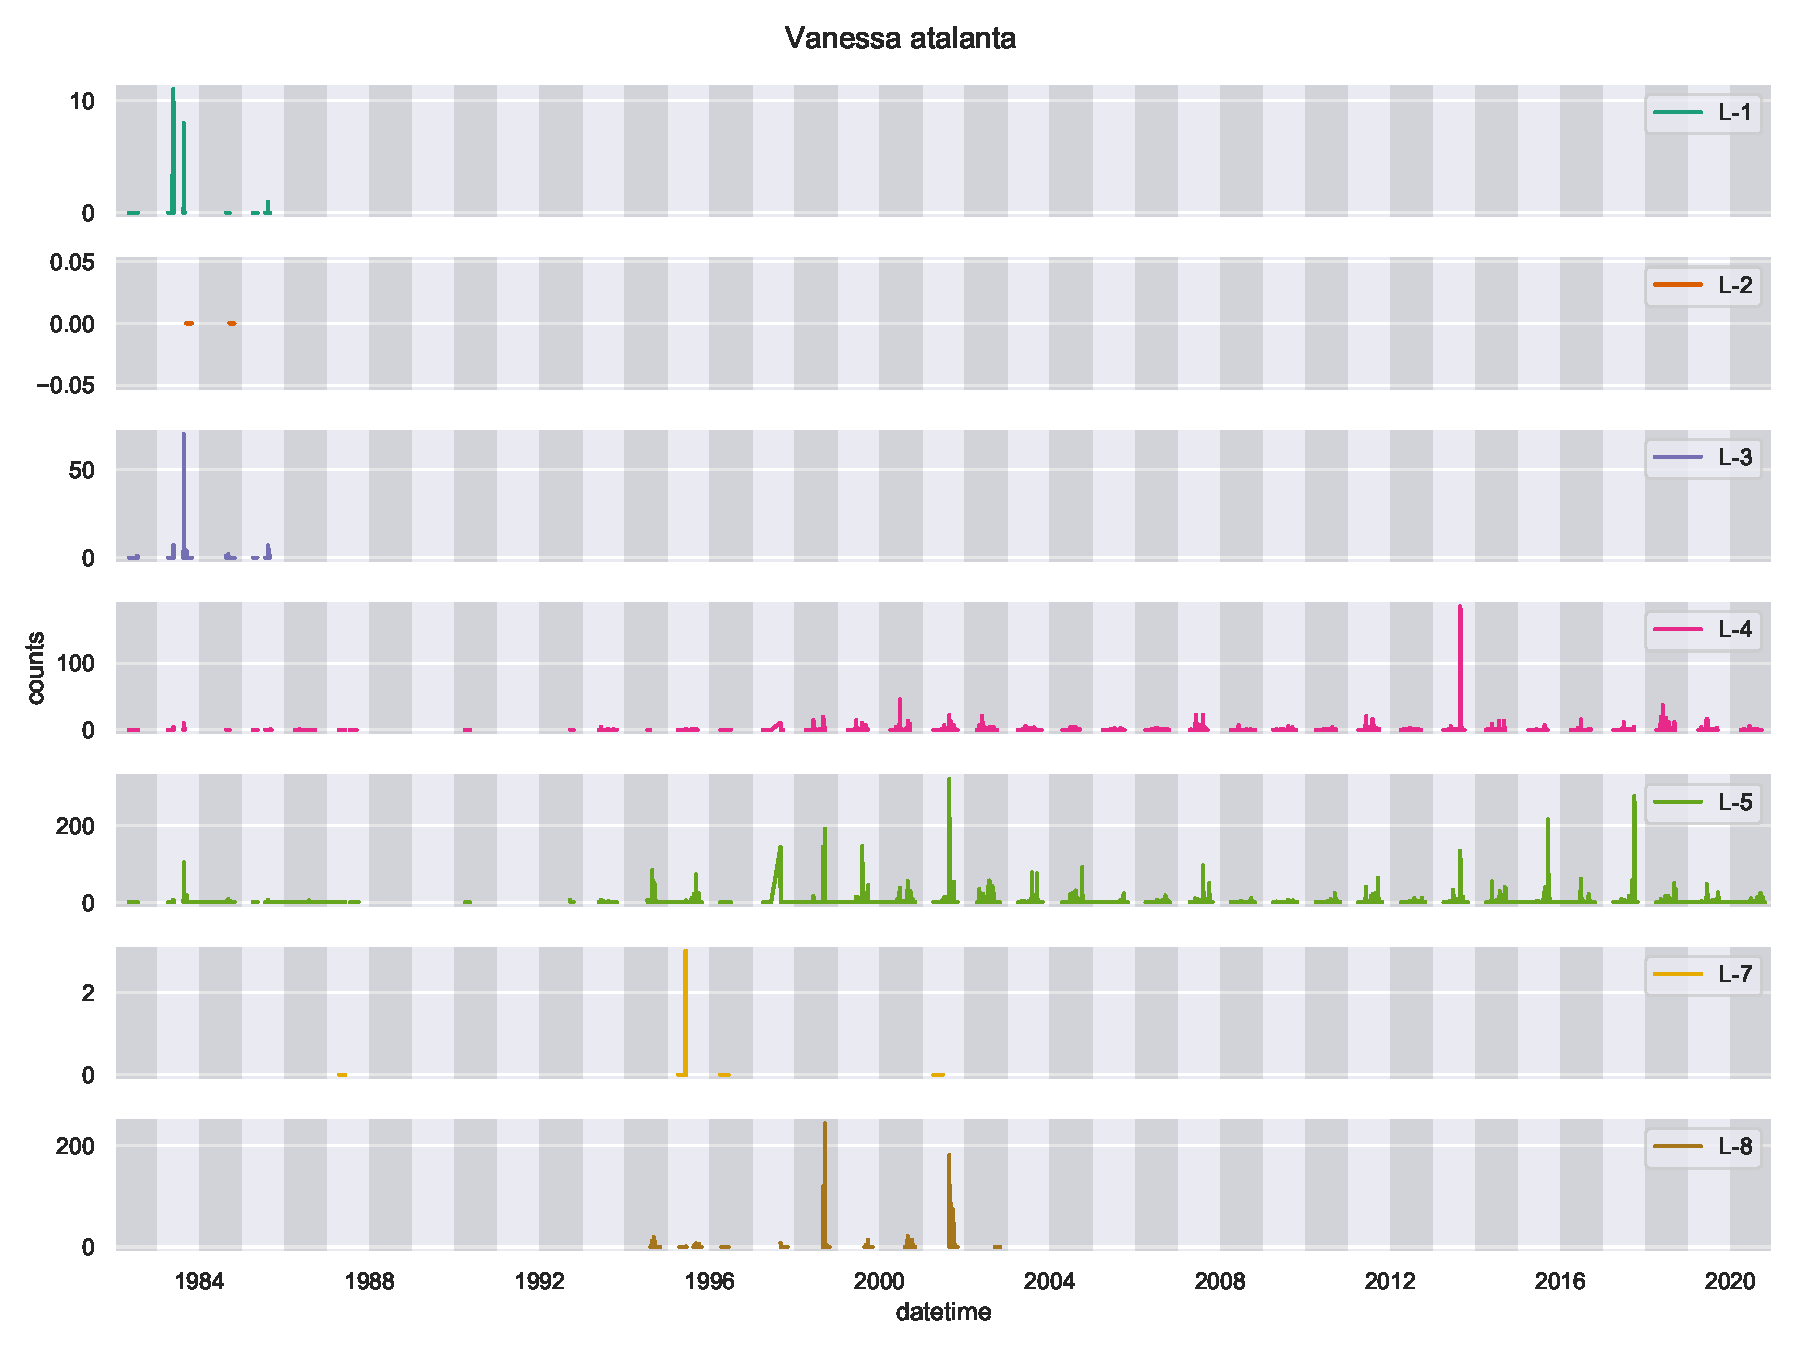
\includegraphics[width=0.9\linewidth]{figs/v-atalanta_single-traps}
	\caption{Daily count of insects caught in individual traps throughout the entire period of time. For illustrative purposes, \textit{V. atalanta} with relatively high abundances was selected, other species can be found \href{https://github.com/gtlab-barcelona/Robert/tree/main/data-exploration_first-last/figs/species_kaliningrad_time-evol_single-traps}{online}. The traps are labelled from \textit{L-1} to \textit{L-8}.}
	\label{fig:v-atalanta}
\end{figure}

%%%

\begin{table}
\centering
\begin{tabular}{@{}ll
		S[table-format=2.1]
		S[table-format=1.3]
		S[table-format=-2.2]
	@{}}
	\toprule
	species & appearance & {\(r^2\) [\%]} & {p-value} & {change (+10y)} \\ \midrule
	Vanessa atalanta & first & 24.0 & \cellcolor{Yellow}0.018 & -13.94 \\
	& last & 1.3 & 0.602 & -1.63 \\
	Vanessa cardui & first & 6.1 & 0.28 & -9.17 \\
	& last & 1.3 & 0.618 & -2.97 \\
	Inachis io & first & 19.7 & \cellcolor{Yellow}0.039 & -4.62 \\
	& last & 0.0 & 0.998 & -0.01 \\
	Issoria lathonia & first & 7.8 & 0.22 & -18.86 \\
	& last & 7.8 & 0.22 & -7.04 \\
	Aglais urticae & first & 12.9 & 0.092 & -28.87 \\
	& last & 0.4 & 0.762 & 1.68 \\
	Aporia crataegi & first & 7.6 & 0.285 & -3.5 \\
	& last & 1.7 & 0.62 & 3.79 \\
	Apatura ilia & first & 9.2 & 0.465 & -5.14 \\
	& last & 94.4 & 0.0 & -41.92 \\
	Aphantopus hyperanthus & first & 3.4 & 0.397 & -2.68 \\
	& last & 4.6 & 0.324 & 2.08 \\
	Araschnia levana & first & 0.2 & 0.884 & 2.66 \\
	& last & 1.4 & 0.686 & 4.49 \\
	Nymphalis antiopa & first & 0.0 & 0.945 & 0.99 \\
	& last & 2.4 & 0.487 & -6.74 \\
	Nymphalis polychloros & first & 12.3 & 0.11 & -15.75 \\
	& last & 1.3 & 0.612 & -6.52 \\
	Nymphalis xanthomelas & first & 14.0 & 0.208 & -32.13 \\
	& last & 0.2 & 0.896 & 3.09 \\
	Papilio machaon & first & 13.0 & 0.276 & -19.57 \\
	& last & 15.6 & 0.23 & 9.84 \\
	Polygonia c-album & first & 20.1 & \cellcolor{Yellow}0.036 & -13.21 \\
	& last & 9.3 & 0.168 & 4.83 \\
	Pararge aegeria & first & 0.4 & 0.81 & 4.11 \\
	& last & 14.1 & 0.138 & -13.05 \\ \bottomrule
\end{tabular}
\caption{Statistical output of regression analysis of linear trend in first and last appearance. The coefficient of determination \(r^2\) is the square of the Pearson correlation \linebreak coefficient. The p-value is derived from a hypothesis test whose null hypothesis is that the slope is zero, using Wald Test with t-distribution of the test statistic. Significance is indicated by yellow filling. Values for change per decade are number of days (\href{https://github.com/gtlab-barcelona/Robert/blob/main/data-exploration_first-last/code/5-stat_output.csv}{csv-file link}).}
\label{tab:stats}
\end{table}

